%% Results chapter
%% author Liu Peng

After designing, implementing and testing the application. We conducted several evaluation tests on the streaming performance. We had released the first edition of the application in Google Play Store in Nov 2013. Since then, we had been updating the application in order to improve its performance and enrich its features. During the past one year, we have collected a big amount of useful data and interesting results. In this chapter we will present and analyze these results.
\subsection{Evaluation of streaming performance}
In terms of streaming, our solution includes two major streaming components. It would be helpful to study and compare which streaming protocol has the better performance while streaming multimedia contents. Moreover, by streaming different types of media and make comparison, we could reveal which protocol is more suitable for a certain type of media. \\
\\The two major streaming technologies we used in our solution are HTTP streaming and RAOP streaming, respectively.\\
\\
Hypertext Transfer Protocol (HTTP) is the protocol used to deliver web pages and images across the World Wide Web. HTTP is a most widely adopted, open standard and the most ubiquitous method of content delivery on the Internet. HTTP objects can be delivered by a variety of web servers, including commercially used servers and open source servers. Both DLNA and Chromecast use HTTP to realize their streaming functionality.\\
\\
Unlike HTTP, another popular protocol, the Real Time Streaming Protocol (RTSP) is a network control protocol used in entertainment and communications systems to control media streaming servers. RTSP is used to establish and control media sessions between two points, usually the server and player client. Clients of media servers issue VCR-like commands, such as PLAY and PAUSE, to facilitate real-time control of playback of media files from the server.  The RAOP protocol, which is virtually another version of RTSP, is used by AirPlay, for the streaming of iTunes music.
\subsubsection{Comparison of AirPlay and DLNA traffic}
Since we have both protocols implemented in our application. We could
compare the performance by streaming the same content to two receivers using the
two different protocols. Typically, DLNA music streaming uses HTTP protocol and
AirPlay music streaming uses ROAP protocol. We selected a mp3 music file and
try to stream it to both an AirPlay Speaker and a DLNA Speaker, and we used
Wireshark running on a rooted Android phone to capture the packets in the
network.
\begin{figure}[hb]
\subfigure[AirPlay]{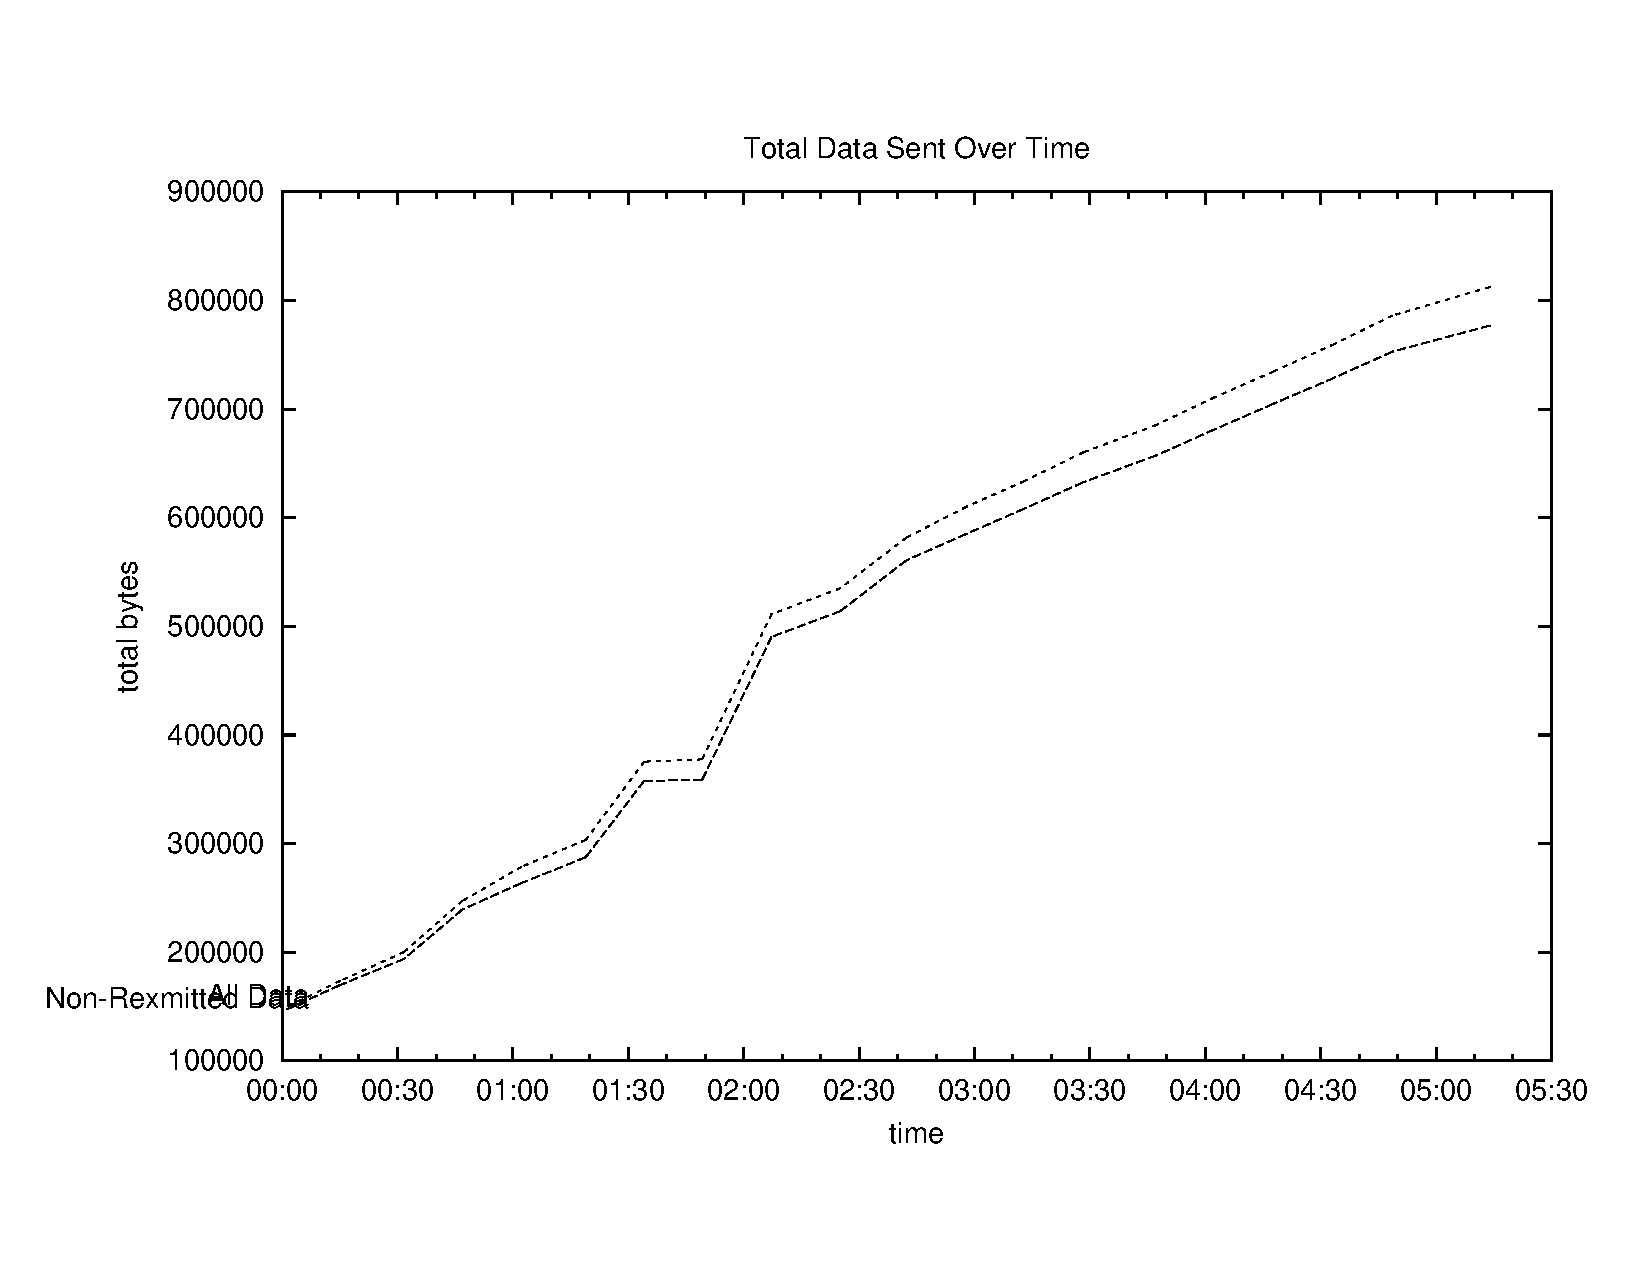
\includegraphics[width=0.9\columnwidth]{charts/oneMoreTime_airplay_android}}
\subfigure[DLNA]{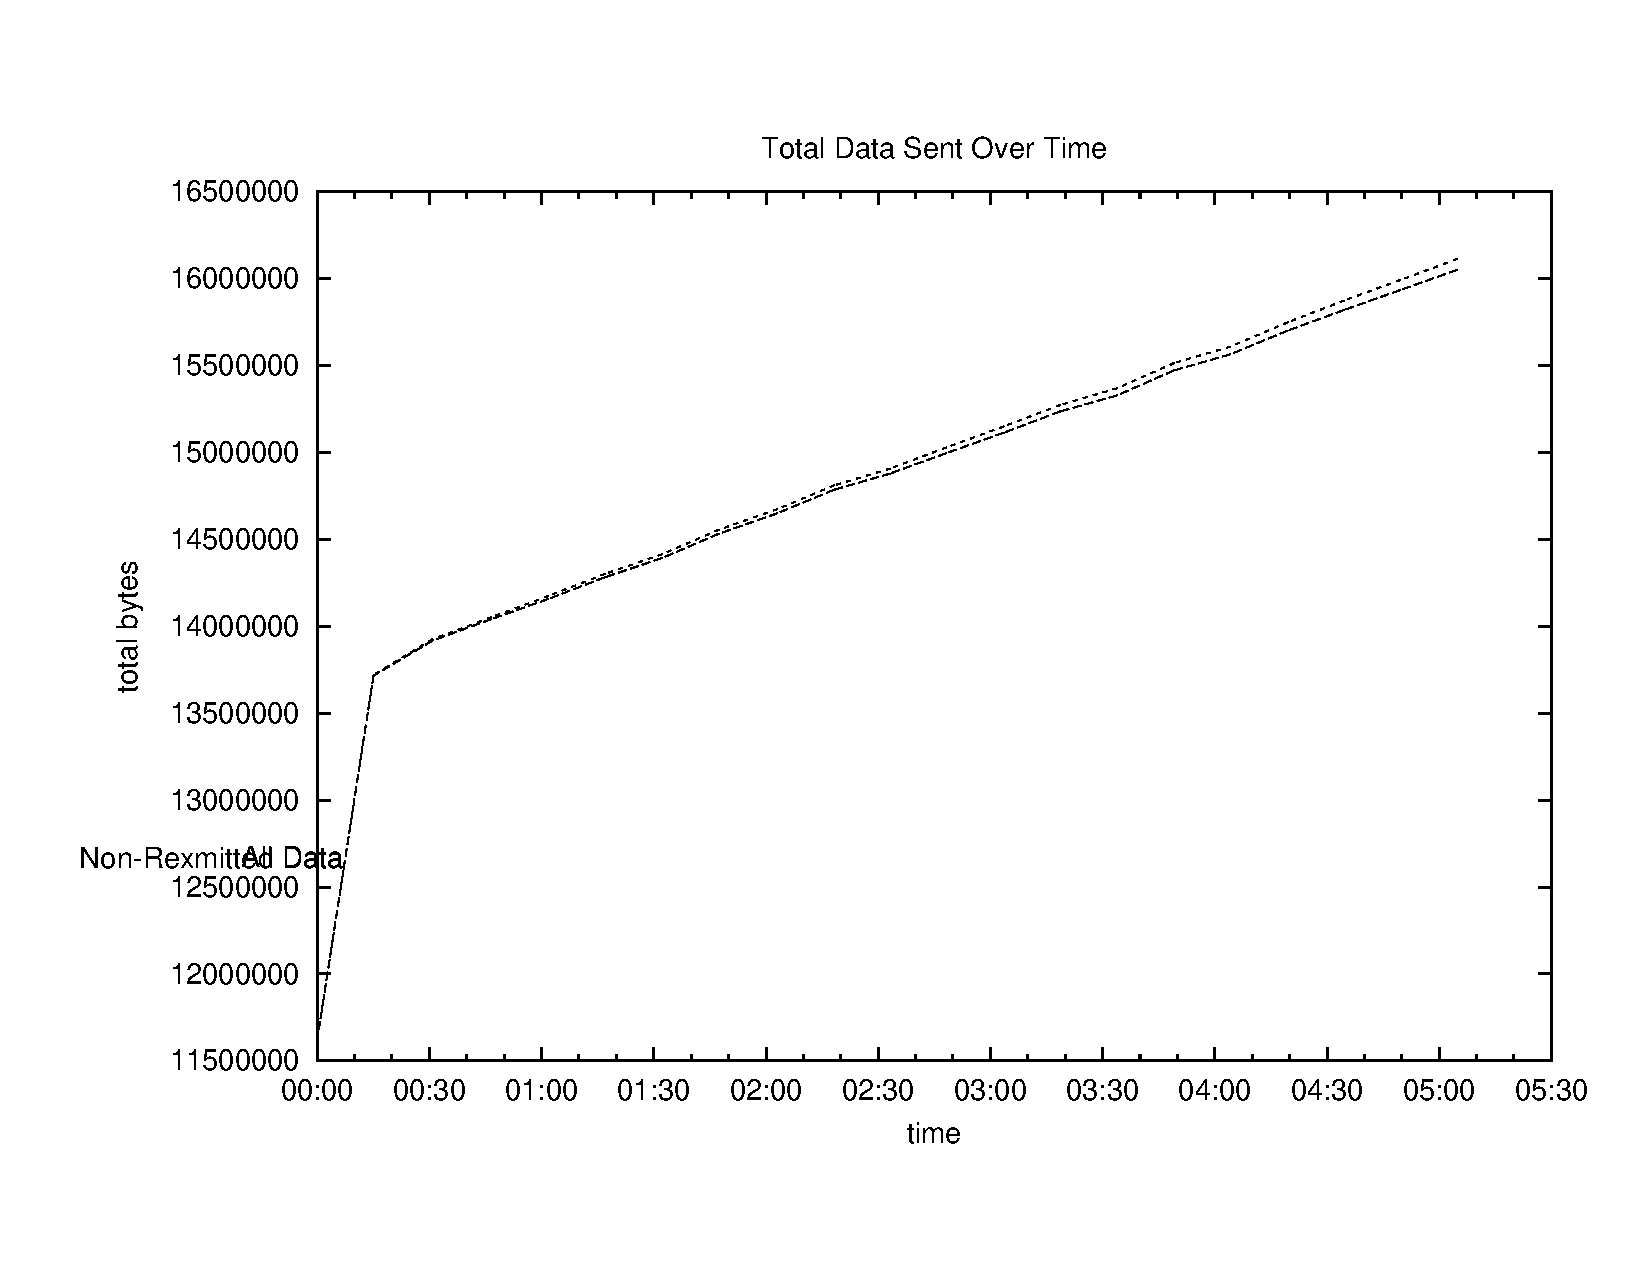
\includegraphics[width=0.9\columnwidth]{charts/oneMoreTime_dlna_android}}
\caption{AirPlay vs DLNA streaming traffic
comparison \label{airplay_vs_dlna_traffic}}
\end{figure}
\clearpage
After the experiment environment is set up, a series of test is conducted and
the result is presented in Figure \ref{airplay_vs_dlna_traffic}.\\
\\
According to the figure, the stream traffics of
AirPlay and DLNA streaming are very different. In AirPlay streaming, the traffic
growth is nearly linear, because ROAP is a push like process and content can be
streamed in real time. However, in DLNA streaming, since its HTTP communication is a pull
like process, the server can actively fetch content from the media server and the content can
be buffered  up since the beginning of the playback, with the best effort of the network.
Therefore, there is a short download period at the beginning of the DLNA
 streaming graph.
\subsubsection{Performance under limited bandwidth }
Then, we evaluate the performance of  the two streaming solutions under limited bandwidth. We limited the bandwidth to 500 kbps, 700 kbps and 1000 kbps respectively and run the streaming. 
During each round of the test streaming, the same mp3 music is streamed to Kodi
using the DLNA standard. Figure \ref{dlna_traffic_bw} and
\ref{dlna_traffic_bw_1} show the result.\\
\\
According to the figure, the initial loading speed is dependent on the bandwidth of network. When there is no limit in bandwidth, the loading speed is the fastest. When the network bandwidth is limited, as the bandwidth of network increases, the initial loading speed would also increase. This proves that in DLNA streaming, most of the content is fully downloaded in the initial phase of streaming,  since HTTP streaming is used. The quality of steaming can be guaranteed when the initial buffering is finished. The receiver will take the buffered content and play locally.\\
\\
In contrast, AirPlay music streaming is based on ROAP, which is a RTP-like protocol. The transport layer protocol used is UDP, thus not all packets are successfully delivered to the receiver. The UDP based delivery only provides a best-effort transmission. The sound quality can not be guaranteed because there is no buffer or retransmission mechanism on the receiver side and the transmission is almost real-time. Given this reason, when the bandwidth is limited to 500 kbps, the AirPlay playback is heavily interrupted. All music information is lost since too many packets are lost during the transmission. When the bandwidth is increased to 700 kbps, the AirPlay playback still can not work properly. The playback is choppy and noisy. After the bandwidth is increased to 1000 kbps, the music can then work smoothly and no noticeable noise can be heard.\\
\\
\begin{figure}[hb]%[!t]%[hb][!b]
\subfigure[No
limit]{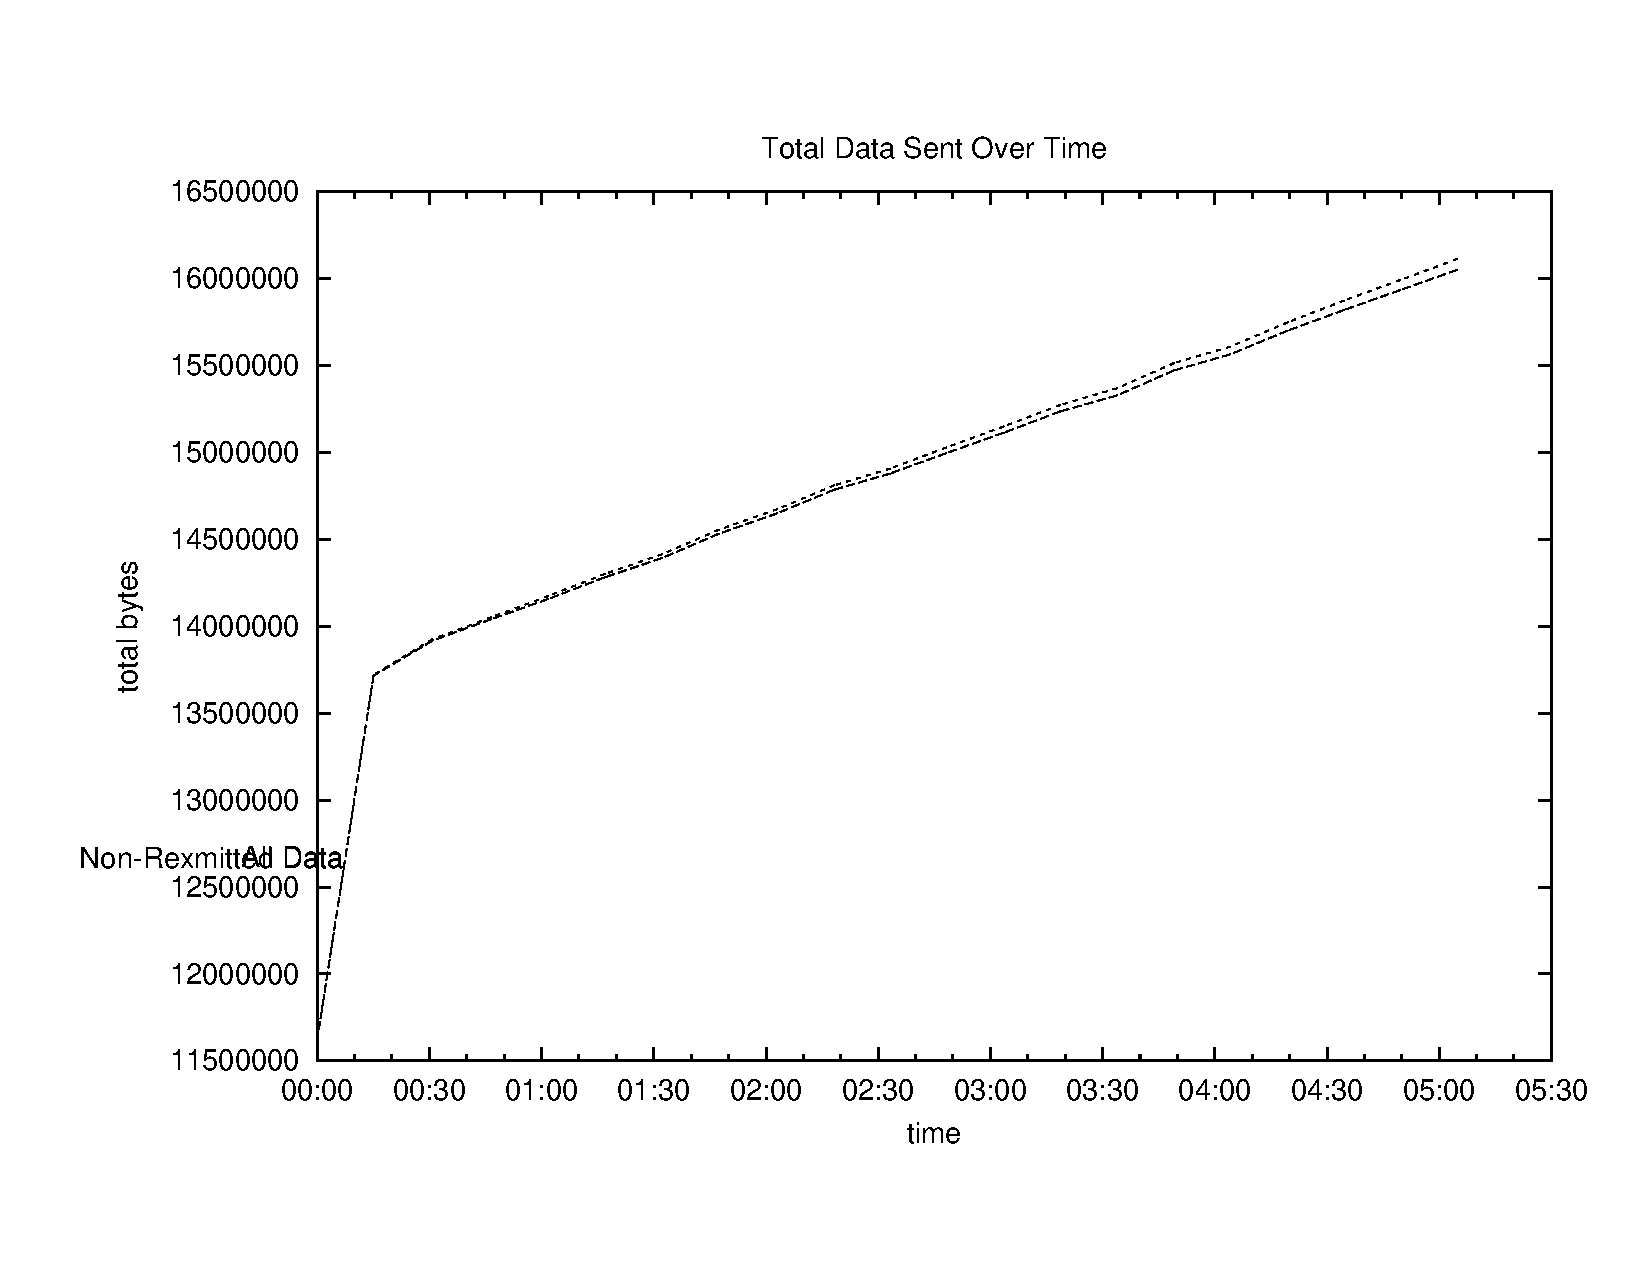
\includegraphics[width=0.9\columnwidth]{charts/oneMoreTime_dlna_android}}
\subfigure[500kbps]{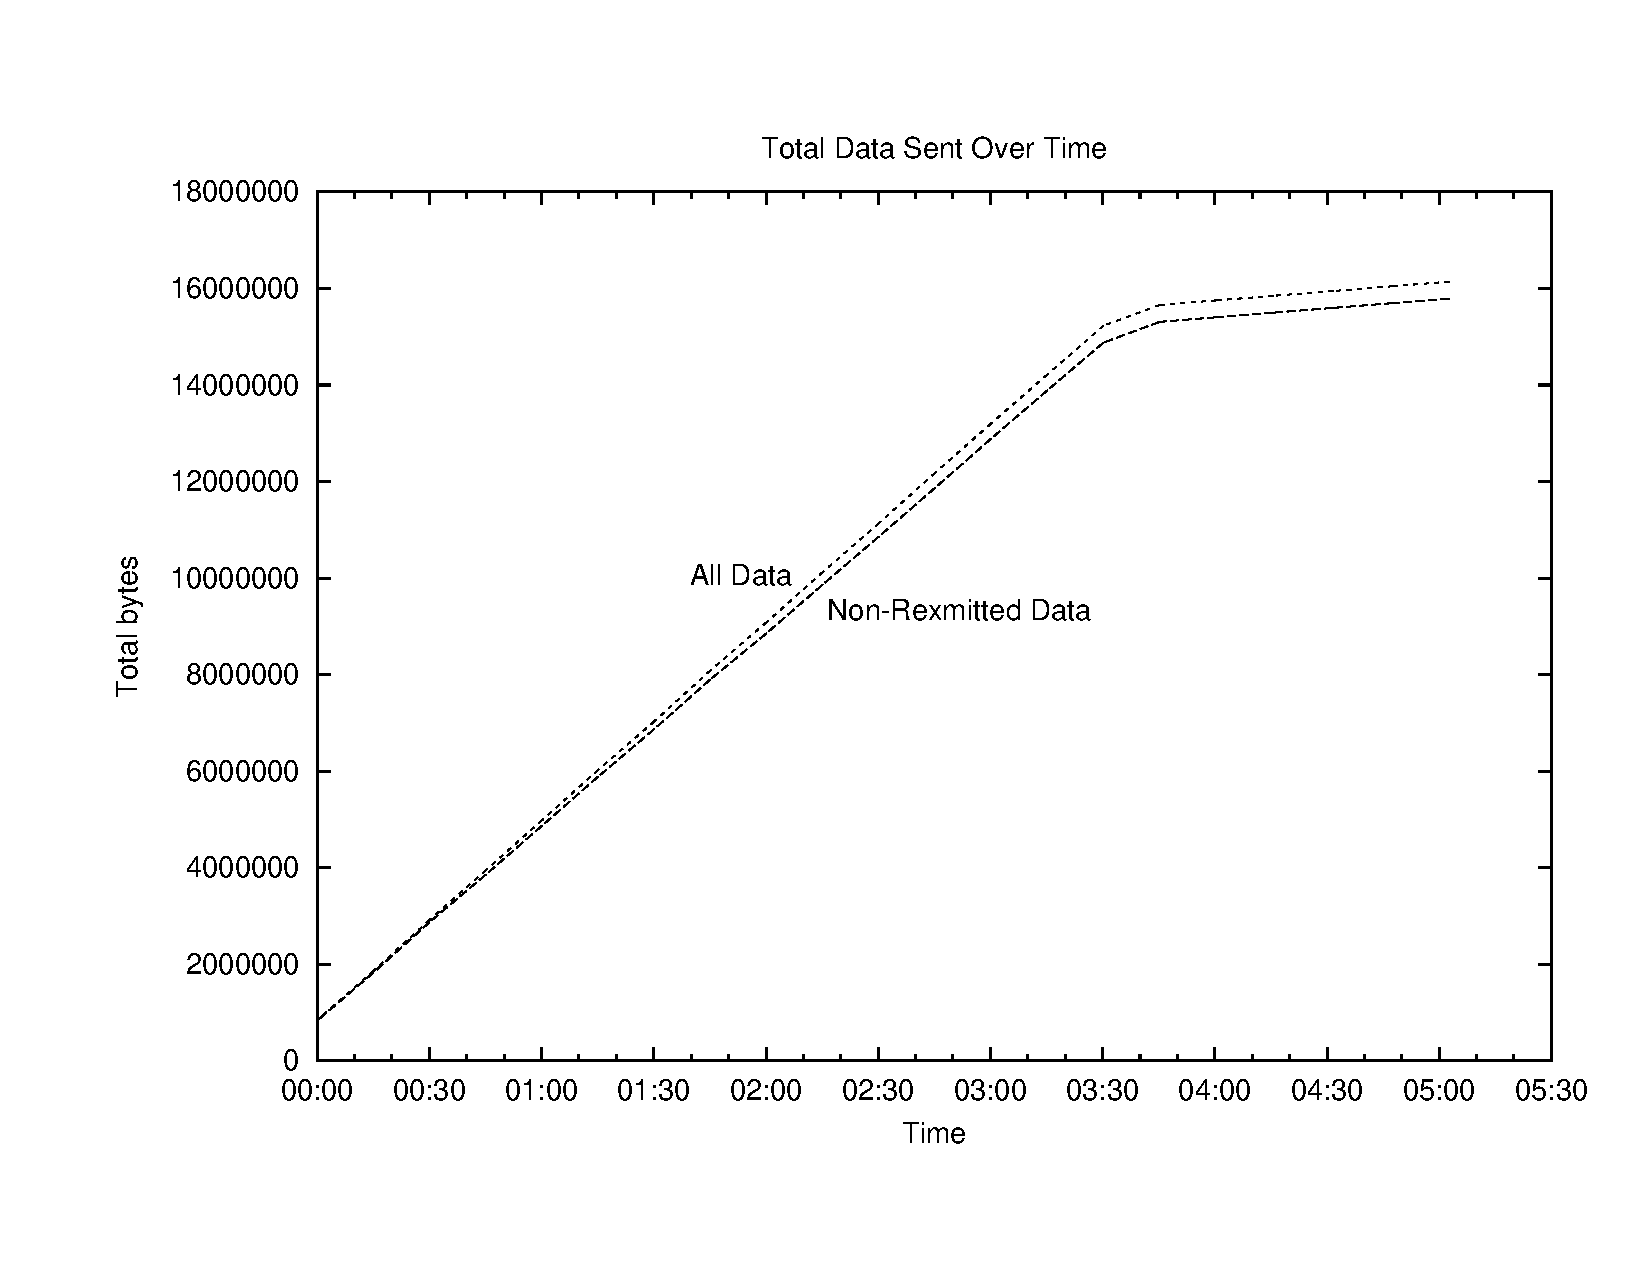
\includegraphics[width=0.9\columnwidth]{charts/oneMoreTime_dlna_android_bw_500k}}
\caption{DLNA streaming traffic comparison in
bandwidth constrained situation\label{dlna_traffic_bw}}
\end{figure}
\begin{figure}[hb]%[!t]%[hb][!b]
\subfigure[700kbps]{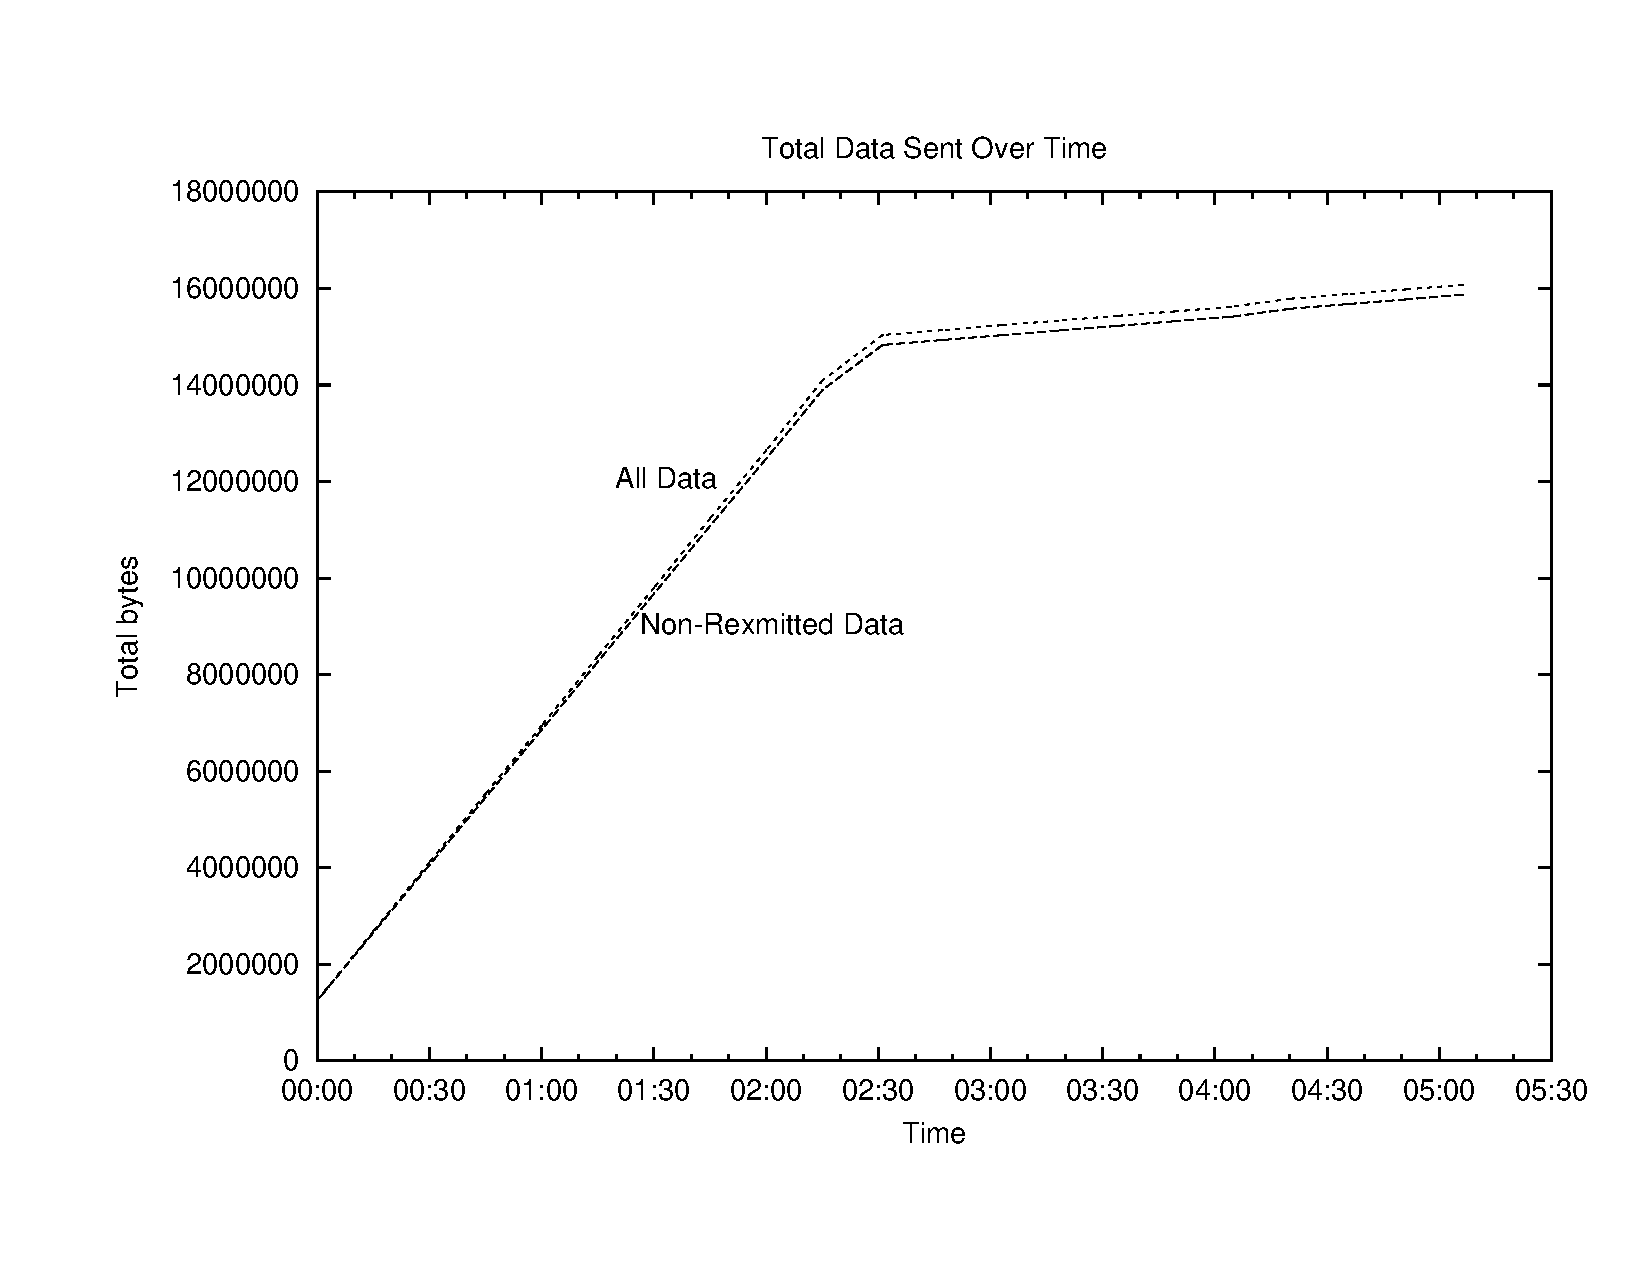
\includegraphics[width=0.9\columnwidth]{charts/oneMoreTime_dlna_android_bw_700k}}
\subfigure[1000kbps]{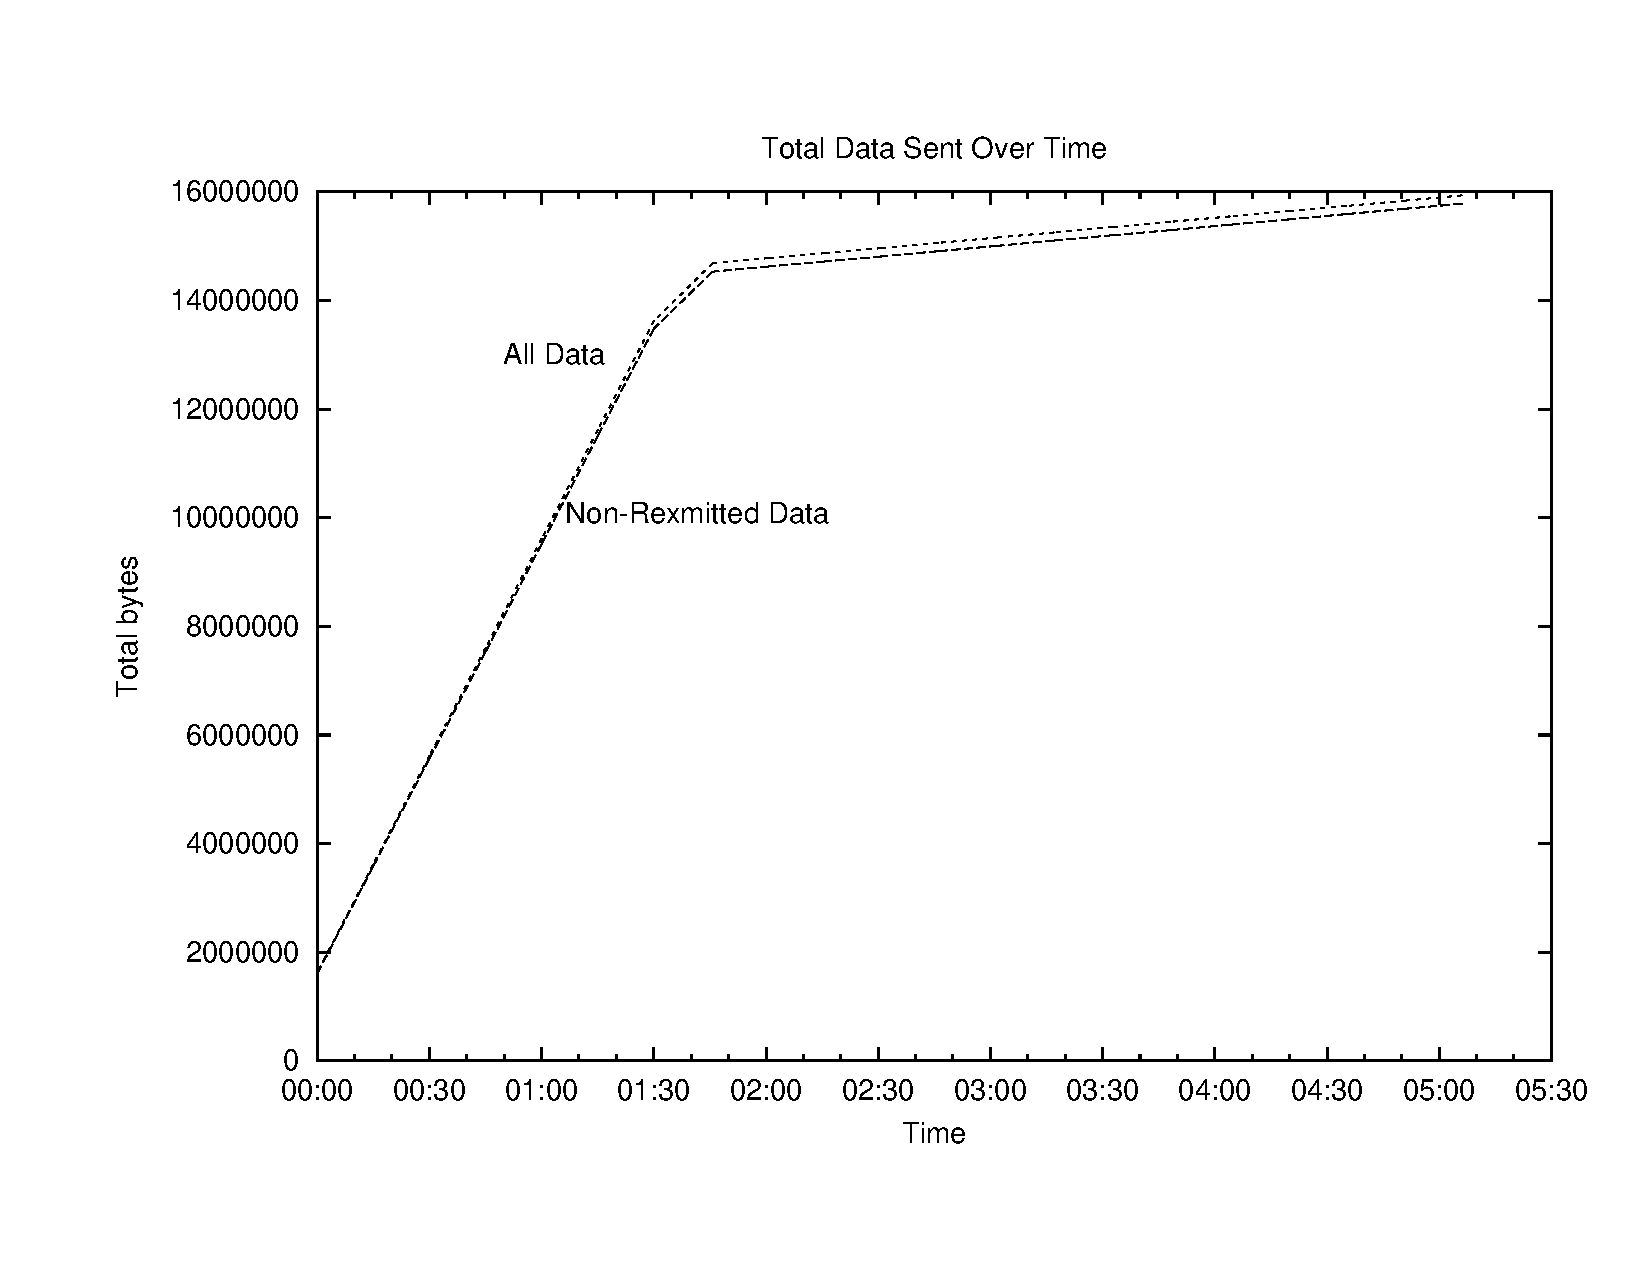
\includegraphics[width=0.9\columnwidth]{charts/oneMoreTime_dlna_android_bw_1000k}}
\caption{DLNA streaming traffic comparison in
bandwidth constrained situation\label{dlna_traffic_bw_1}}
\end{figure}
\clearpage
Another thing worth mentioning is that in the experiment, the same mp3 music is used in both tests. But obviously the playback quality of DLNA is better than the playback using AirPlay. For instance, when the bandwidth is limited to 500 kbps, AirPlay streaming is basically not usable any more, while DLNA streaming is still working properly. The reason behind this is that in the case of DLNA streaming, the original mp3 music is directly streamed to receiver, while in the case of AirPlay music streaming, the same mp3 music is firstly decoded to PCM format and then encoded to Apple Lossless format. Since mp3 is a compressed media format while Apple lossless format is an uncompressed media format, the bandwidth required by DLNA streaming is considerably smaller than AirPlay streaming.\\
\\
Generally speaking, DLNA is more tolerant than AirPlay streaming in the case of limited bandwidth.
\subsubsection{Influence of packet loss}
After the bandwidth test, we then simulated packet loss on the receiver side and
conducted the same test for DLNA and AirPlay streaming. 5\%, 10\% and 15\%
packet loss are introduced to test both DLNA and AirPlay streaming. The result
of DLNA streaming is shown in Figure \ref{dlna_pl} and \ref{dlna_pl_1}.
\begin{figure}[hb]
\subfigure[No
limit]{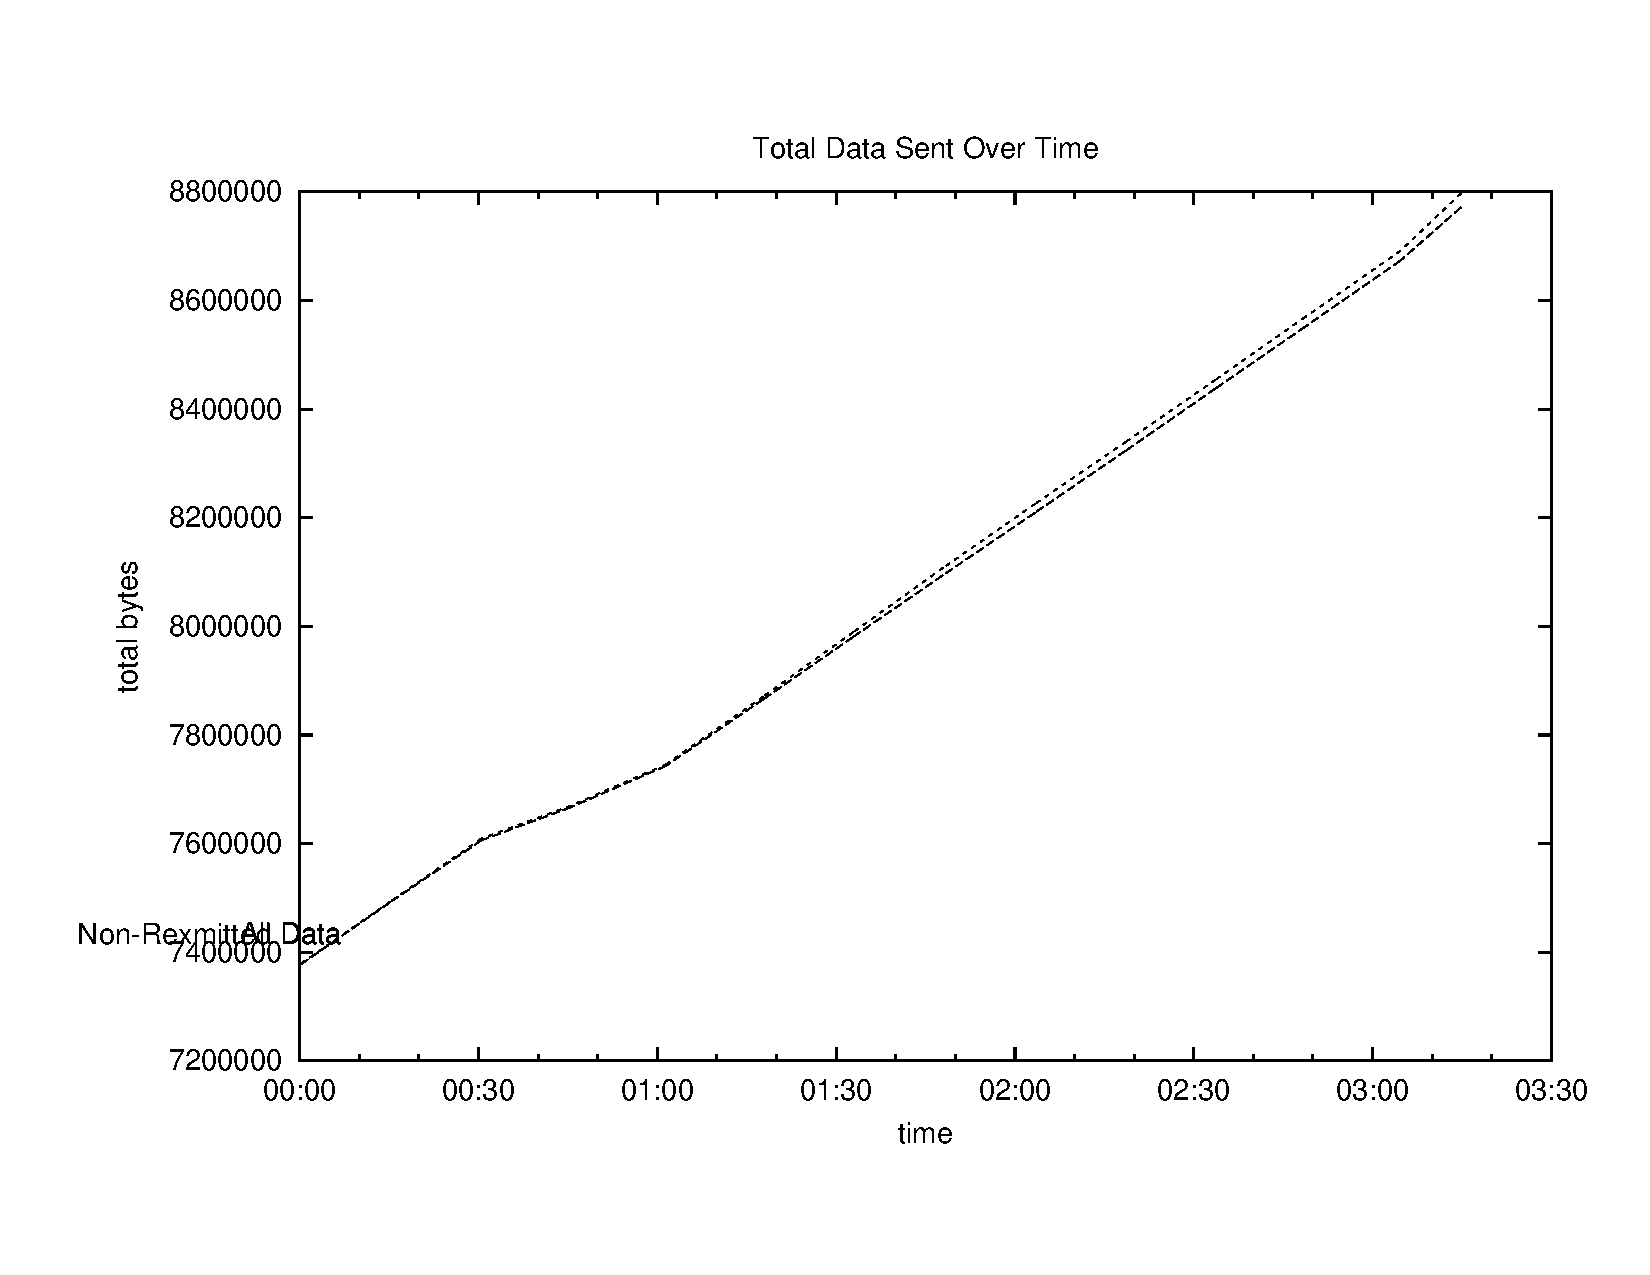
\includegraphics[width=0.9\columnwidth]{charts/dlna_traffic_data}}
\subfigure[5
percent loss]{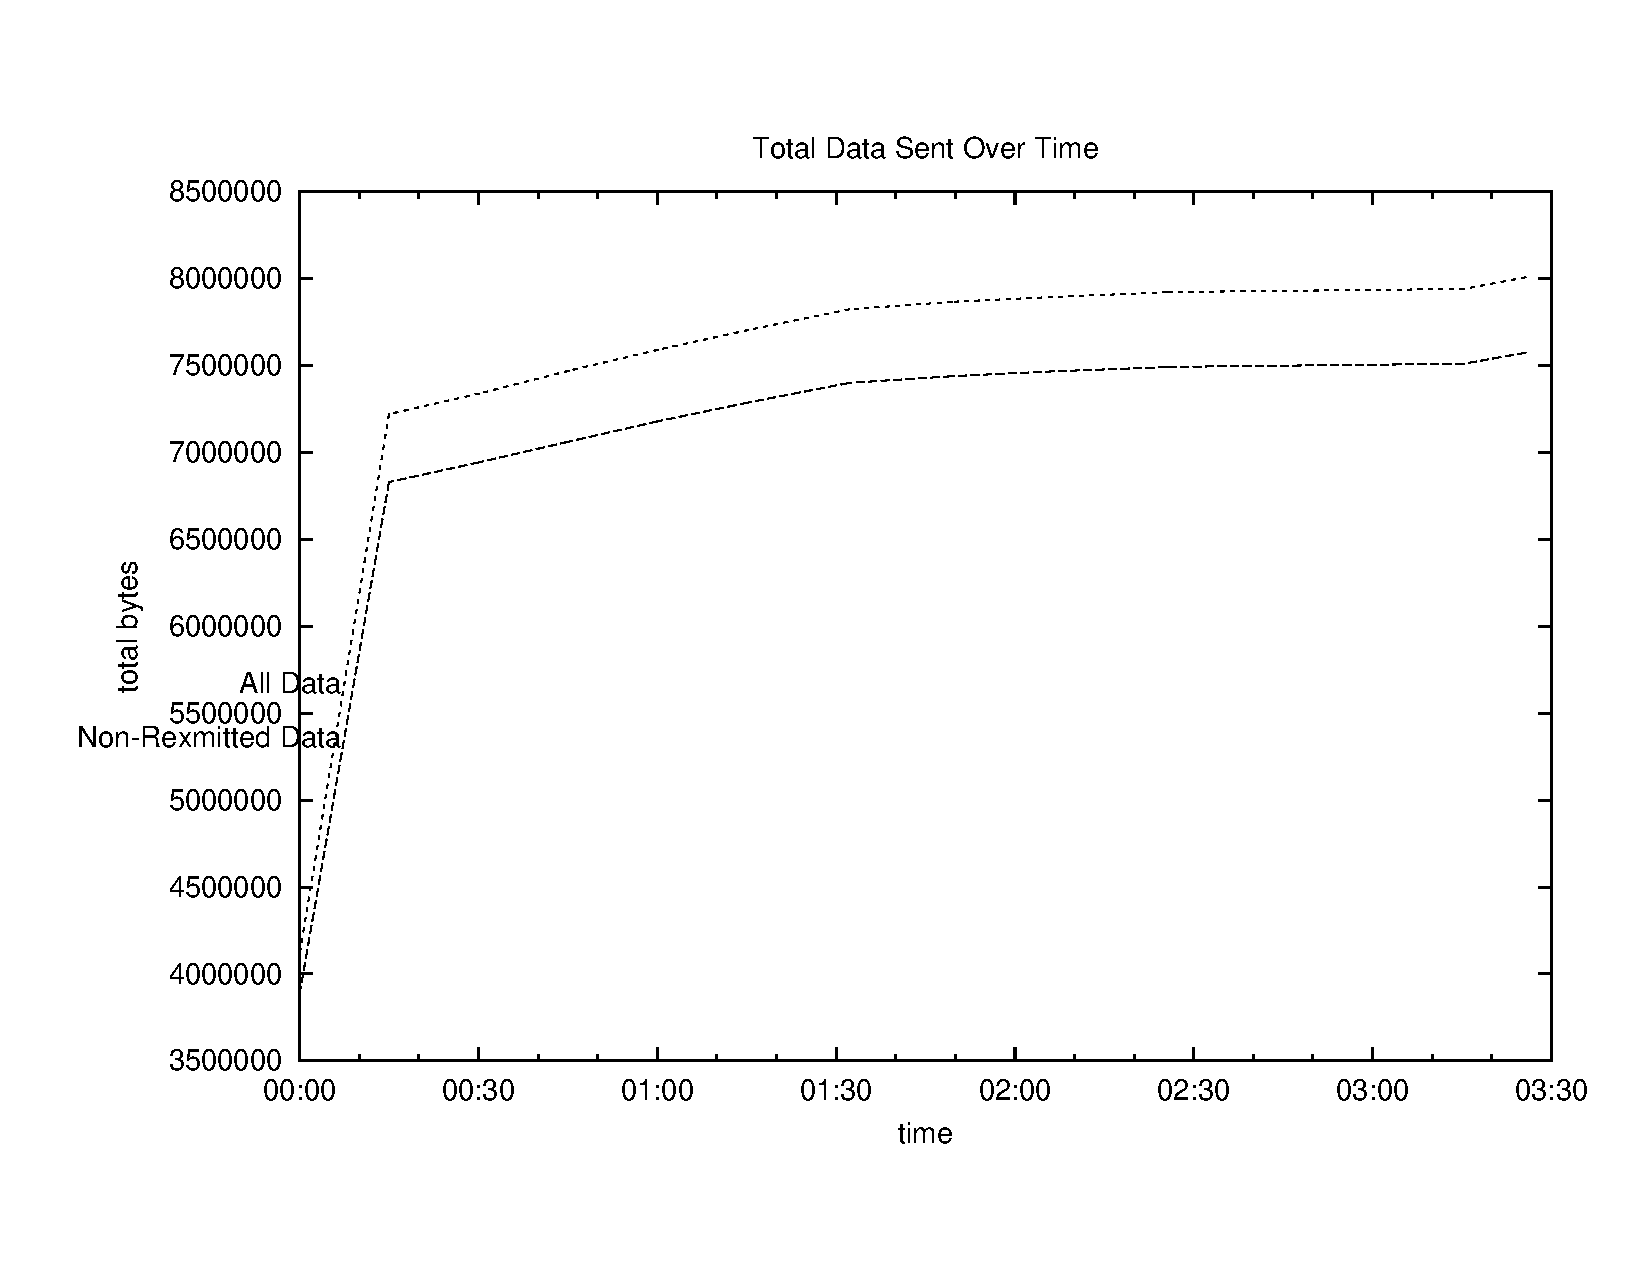
\includegraphics[width=0.9\columnwidth]{charts/dlna_traffic_5loss_data}}
\caption{DLNA streaming performance in terms of packet loss \label{dlna_pl}}
\end{figure}

\begin{figure}[hb]
\subfigure[10
percent loss]{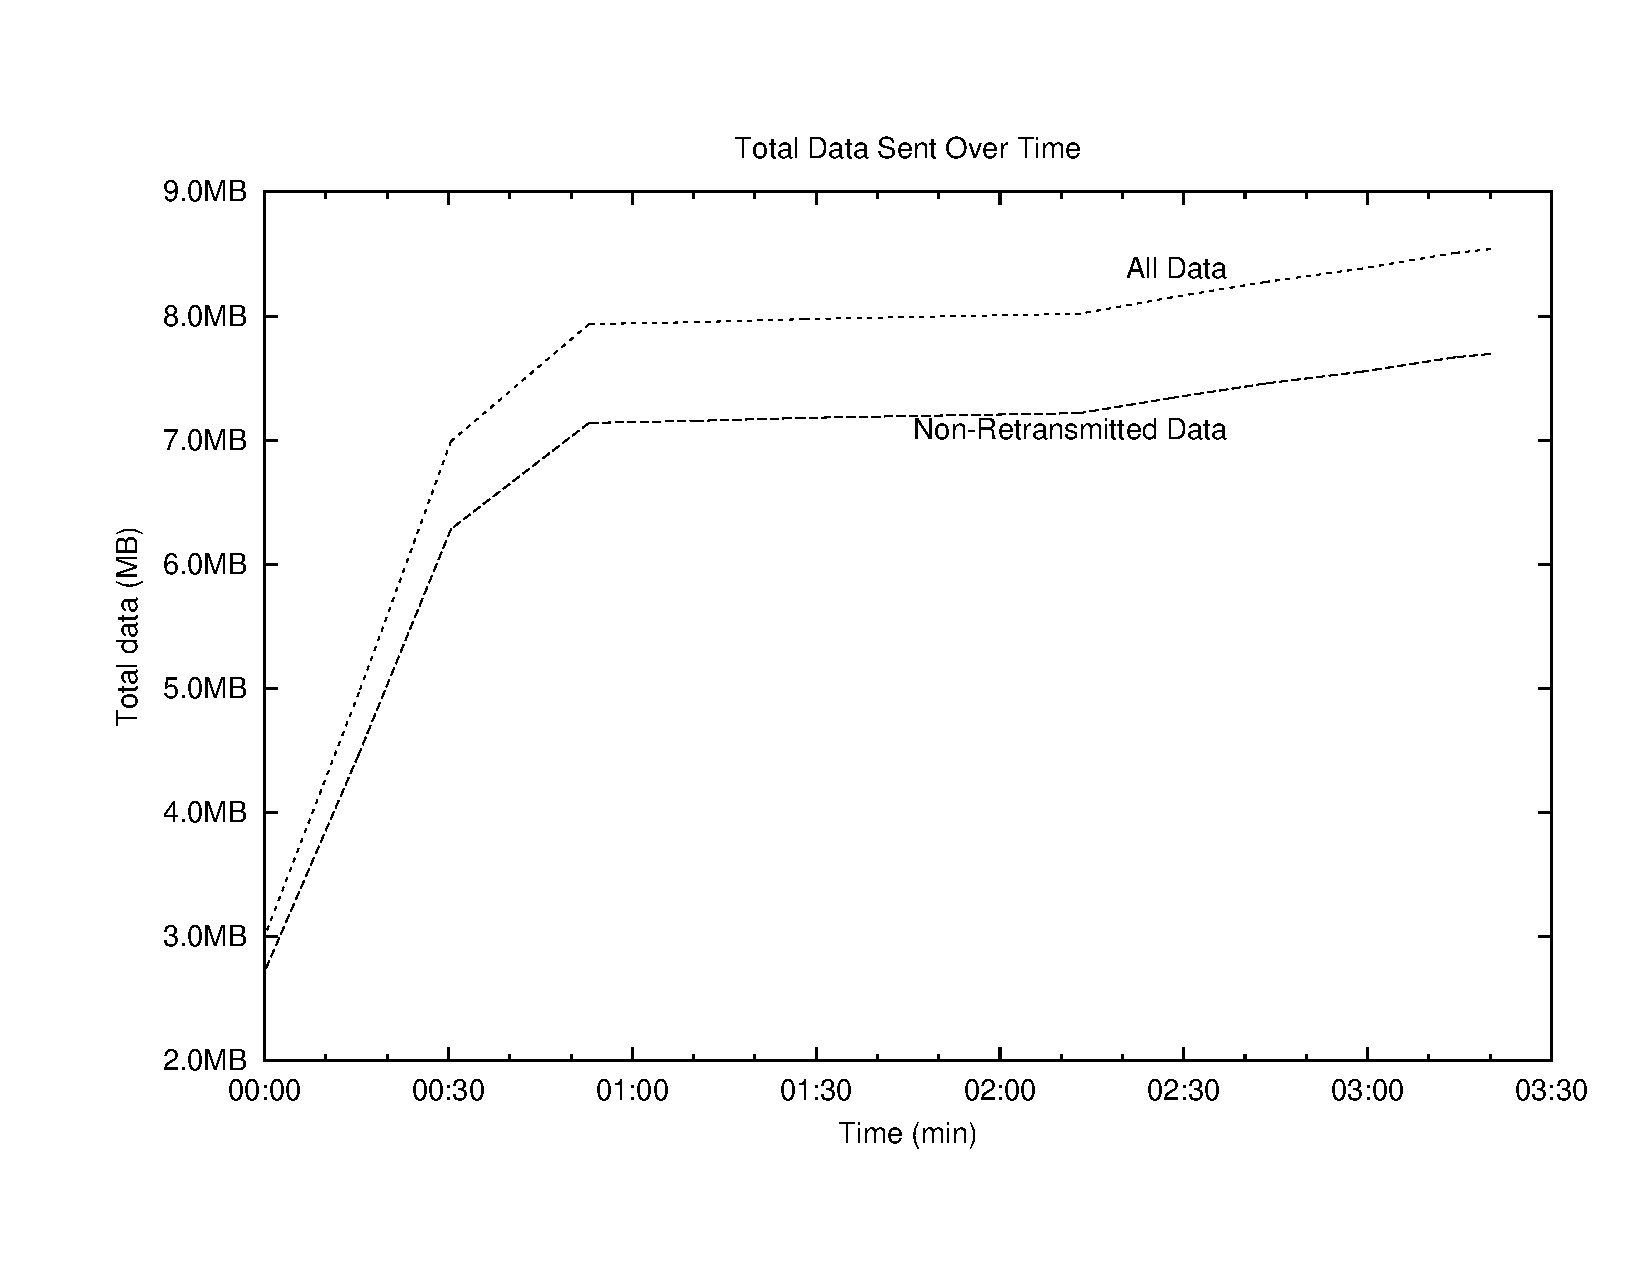
\includegraphics[width=0.9\columnwidth]{charts/dlna_traffic_10loss_data}}
\subfigure[15
percent loss]{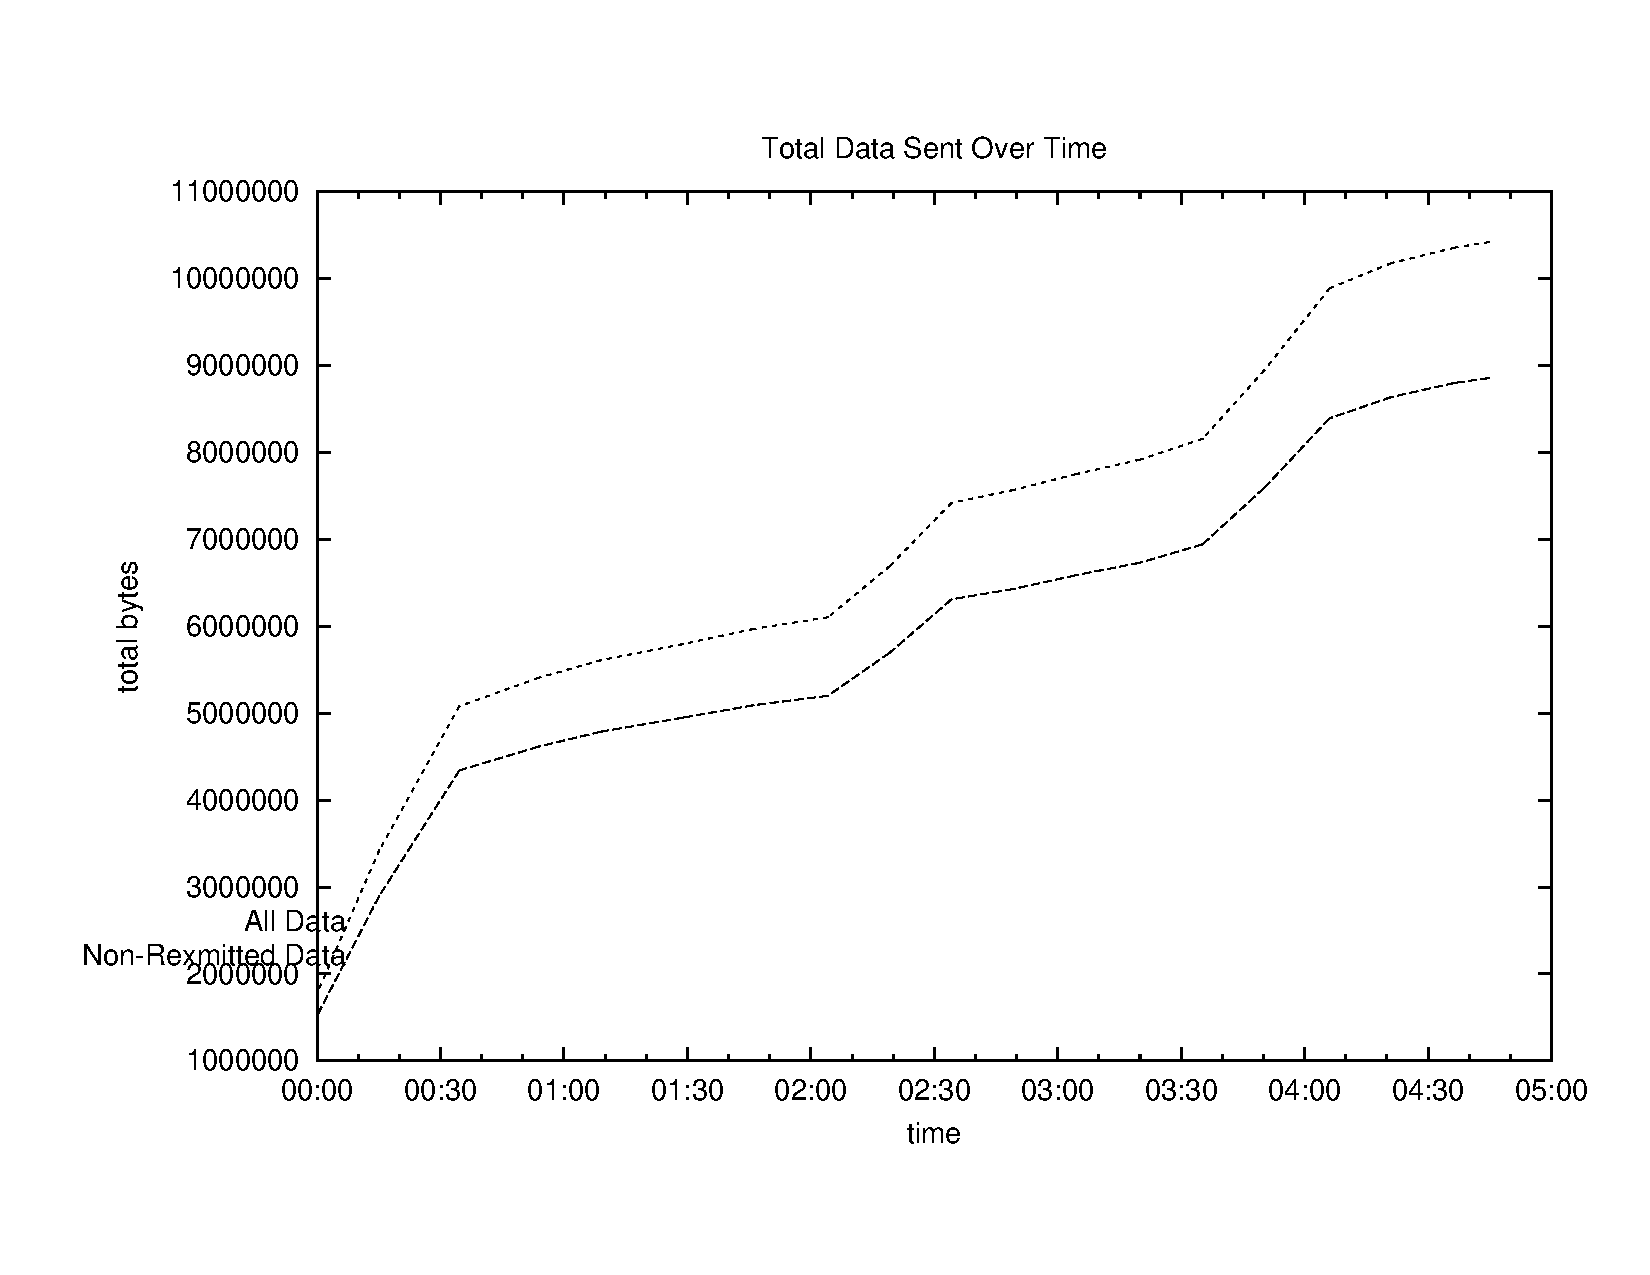
\includegraphics[width=0.9\columnwidth]{charts/dlna_traffic_15loss_data}}
\caption{DLNA streaming performance in terms of packet loss \label{dlna_pl_1}}
\end{figure}
According to the figure, when there is no packet loss, very little retransmission data is seen in the graph. When the packet loss ratio is increased from 5\% to 10\%, the portion of retransmitted data is getting larger and larger. However, there is no noticeable loss of sound quality. When the packet loss ratio is increased to 15\%, significant amount of retransmission can be found in the graph, and the streaming stopped for buffering three times during one song's playback. In the case of DLNA streaming, packet loss is a key impediment. When packet loss rate climbs to a certain point, for instance 15\% in our test, the streaming becomes unusable.\\
\\
The same packet loss tests on AirPlay streaming was also conducted and the
results are shown in Figure \ref{airplay_pl} and \ref{airplay_pl_1}. According
to the figure, in the case of AirPlay streaming, since UDP is used, the ROAP server embedded in Streambels keeps sending data to the receiver using UDP regardless of  the packet loss. On the receiver side, the player tries its best to decode the broken data. There is no mechanism for acknowledgement or retransmission. Surprisingly, the sound quality is much better compared with DLNA streaming. The reason behind is that retransmission of TCP consumes more and more bandwidth in the case of DLNA streaming, in the same situation. AirPlay streaming instead tries to deliver all contents with its best effort, without creating extra demand for retransmission.\\
\\
In a nutshell, in the case of packet loss, AirPlay is more tolerant to packet loss than DLNA.
\begin{figure}[hb]
\subfigure[No
limit]{\includegraphics[width=0.9\columnwidth]{charts/AirPlay_traffic_data}}
\subfigure[5
percent loss]{\includegraphics[width=0.9\columnwidth]{charts/AirPlay_traffic_5loss_data}}
\caption{AirPlay streaming performance in terms of packet loss \label{airplay_pl}}
\end{figure}
\begin{figure}[hb]
\subfigure[10
percent loss]{\includegraphics[width=0.9\columnwidth]{charts/AirPlay_traffic_10loss_data}}
\subfigure[15
percent loss]{\includegraphics[width=0.9\columnwidth]{charts/AirPlay_traffic_15loss_data}}
\caption{AirPlay streaming performance in terms of packet loss
\label{airplay_pl_1}}
\end{figure}
\clearpage

\subsection{Statistics}
16 months after its release, our application has achieved 924000 downloads from 223 countries all around the world, with a daily active user number of over 15000. Our users almost cover 99\% of all continent and a world map of our user distribution is shown in Figure \ref{user_map}. 
\begin{figure}[hb]
\centering 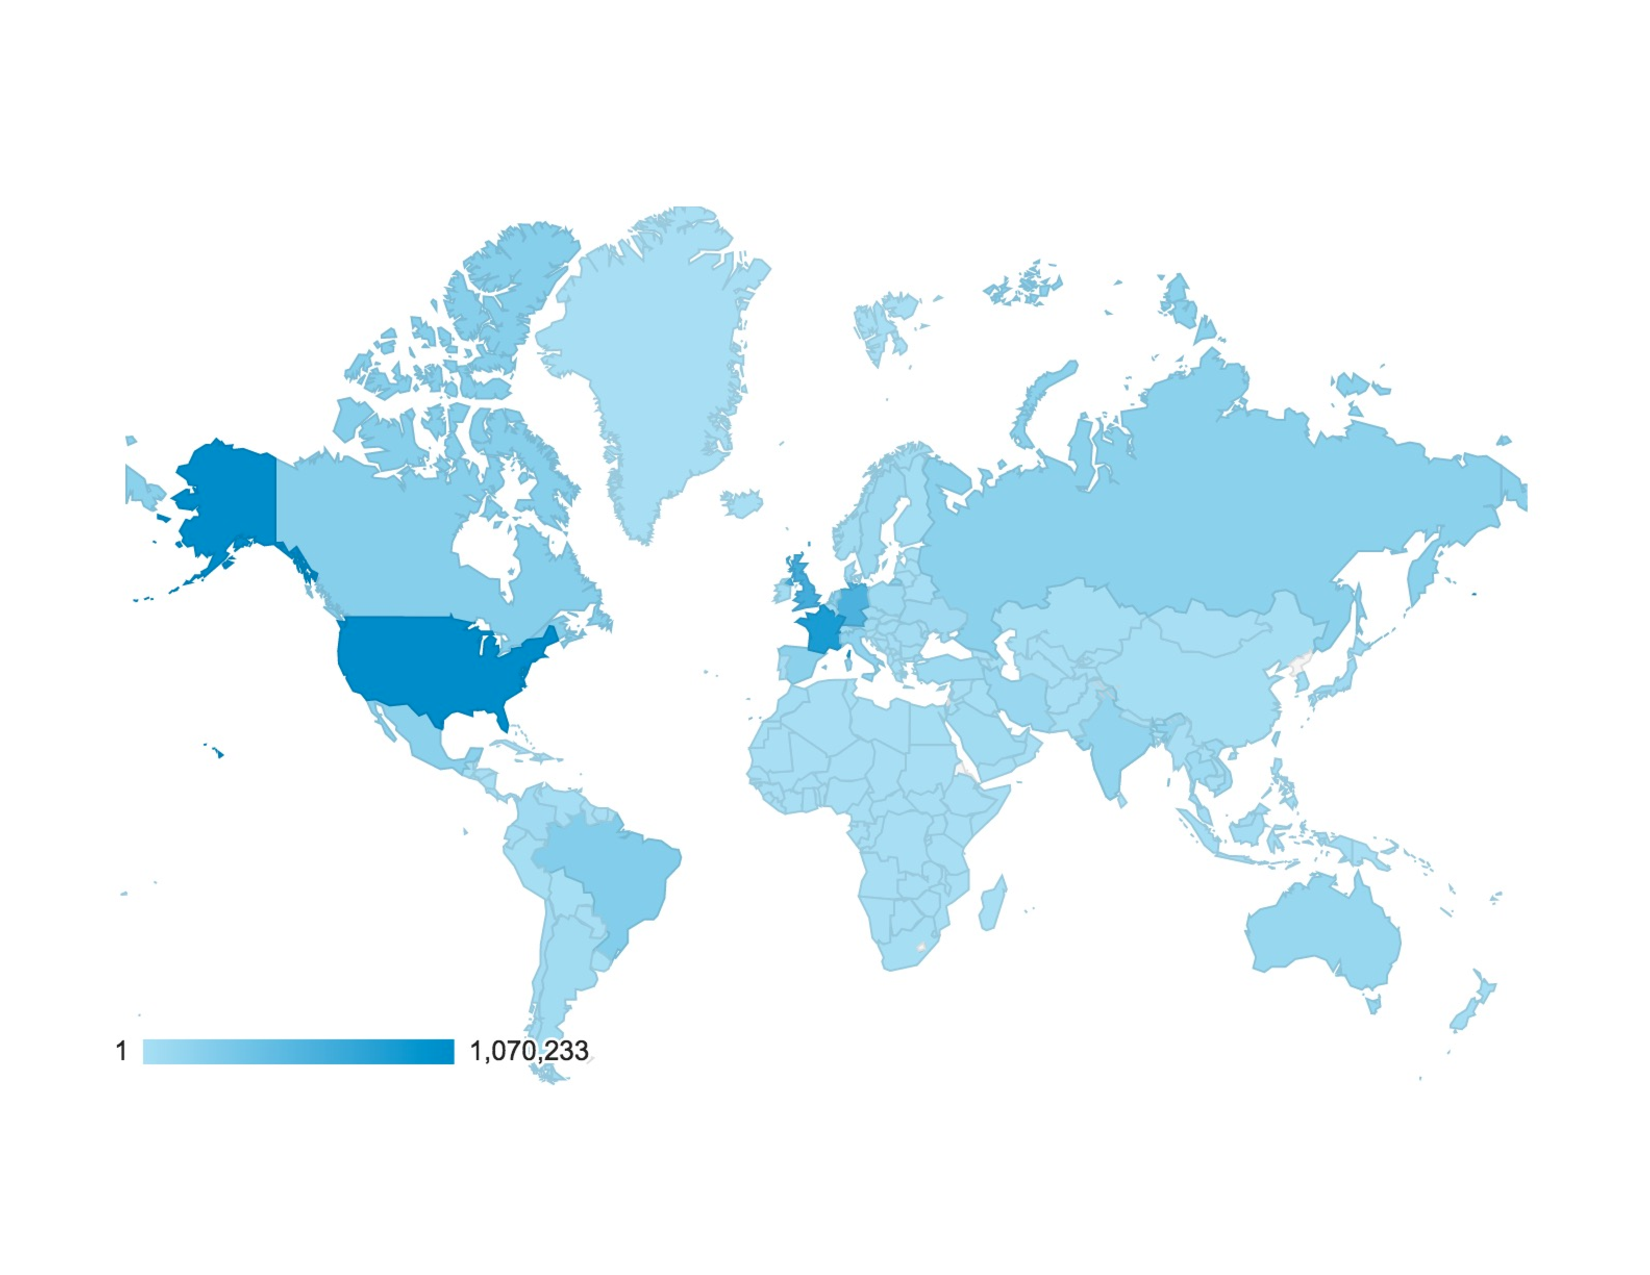
\includegraphics[width=0.9\columnwidth]{charts/session_world_map}
\caption{World map of visits \label{user_map}}
\end{figure}
So far, we have received ratings from 10253 users and currently the average rating is 3.9 out of 5. The distribution is shown in Figure \ref{ratings}. According to the rating distribution graph, most users are satisfied with our solution and give the 5 stars rating. However, the average rating is heavily influenced by the 1 star rating users. The reason for those low ratings is that the receivers some users have in home are not compatible with our application due to different reasons. It might be that some protocols,such as Roku box, are not supported yet. Network condition problem also contributes to the incompatibility issues. For example some routers have by default disabled multicast due to security reasons. Another major cause of the incompatibility problem is that even with the same protocol, such as DLNA , a minor implementation difference may cause the break of connections. Thus, in the later phase, we have made receiver specific hacks to make our application work with most DLNA receivers, regardless of which implementation they use.
\begin{figure}[!t]
\centering 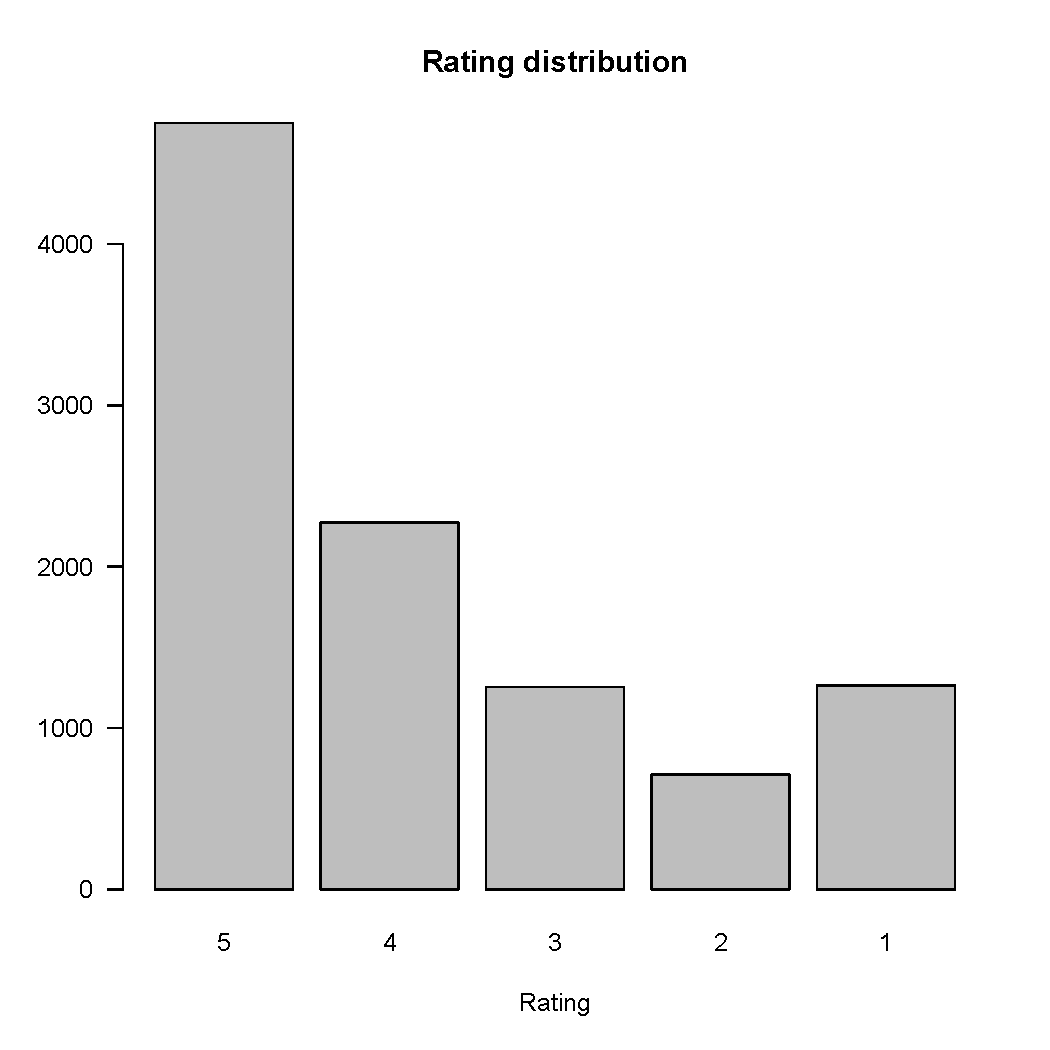
\includegraphics[height=8.5cm]{charts/rating_distribution}
\caption{Rating distribution\label{ratings}}
\end{figure}
In terms of user distribution, in the last 16 months, our application turns out
to be very popular in countries like France, United States, Germany, United Kingdom
and Brazil. The user distribution is shown in Figure \ref{user_country}.
\begin{figure}[htb]
\centering 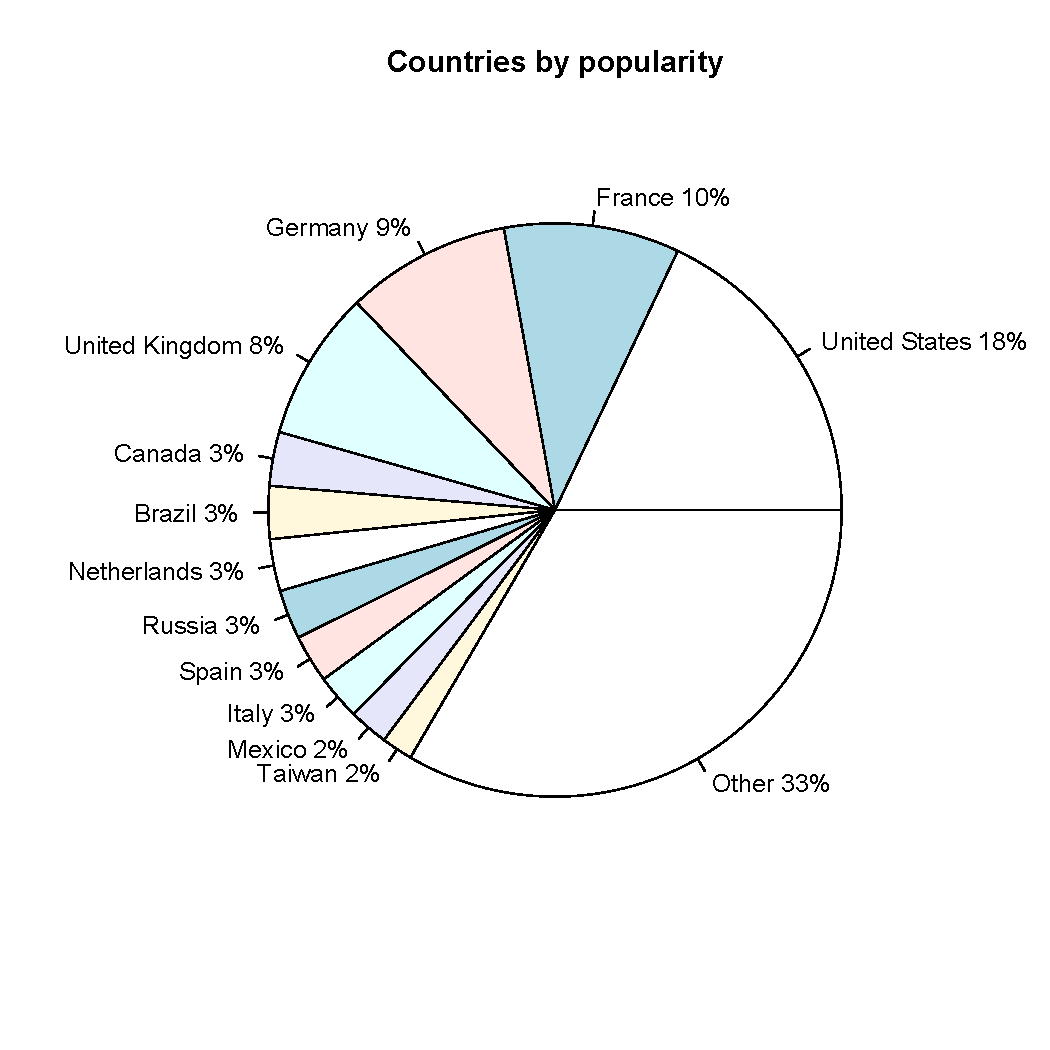
\includegraphics[height=8.5cm]{charts/country_popularity}
\caption{Popularity in different countries \label{user_country}}
\end{figure}
We have also translated the description of our application to nine languages, which include English, Russian, German, Italian, Japanese, French, Chinese, Spanish and Korean. The multiple language support may also contribute to the popularity of our application in all parts of the world.
\begin{figure}[!t]
\centering 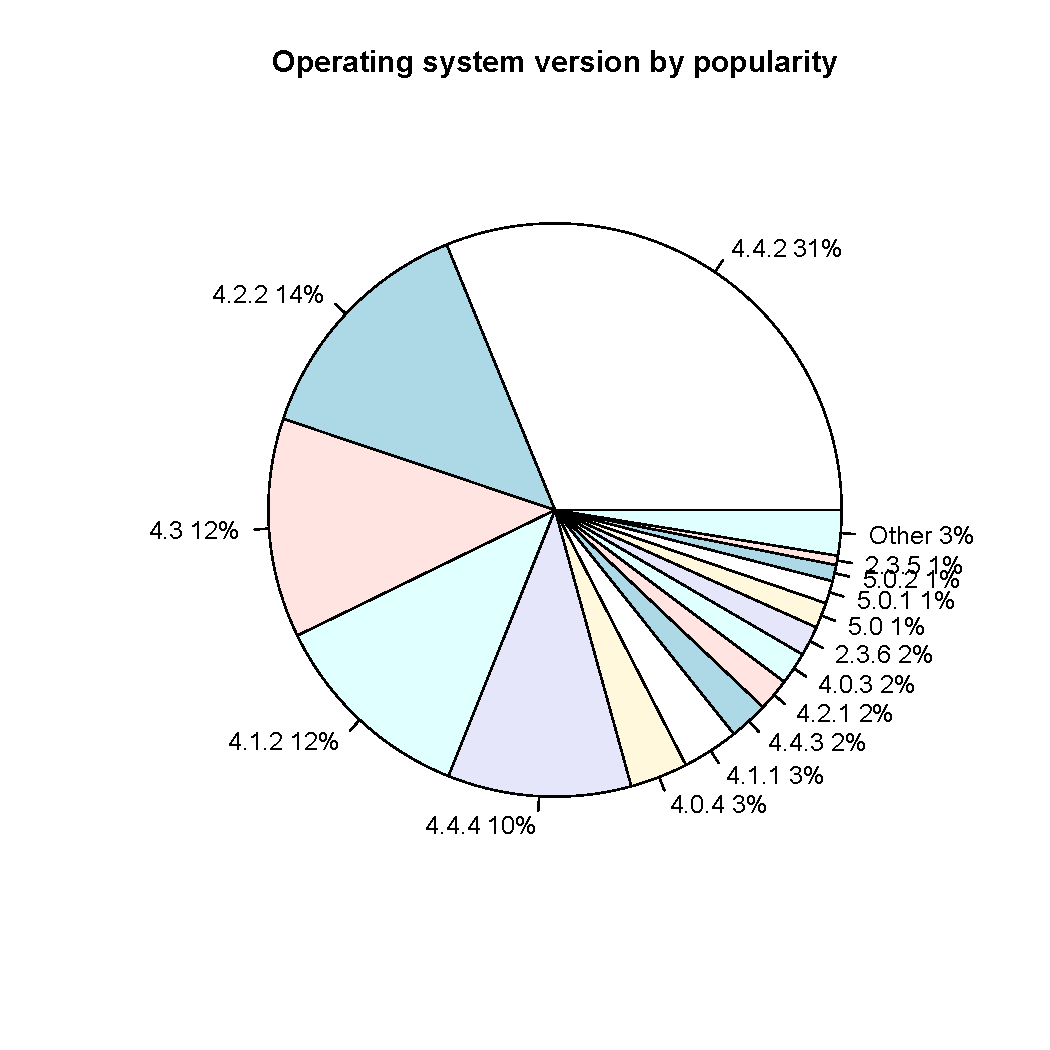
\includegraphics[height=8.5cm]{charts/os_version_popularity}
\caption{Popularity of different Android versions \label{os_versions}}
\end{figure}
The most popular operating system used for our application is Android, but interestingly there are also tens of users was using our application on BlackBerry \footnote{\url{https://developer.blackberry.com/playbook/android/files/webinars/BlackBerry_Runtime_for_Android_Apps.pdf}}, which is another mobile operating system developed by BlackBerry Inc.  For all the users on Android system, the distribution is shown in Figure \ref{os_versions}. According to the statistics, Android Kitkart is the most widely used Android version, which is also our target system version. Most users have updated to the Kitkart version 4.4. We also have a very small part of users who are using the latest Android 5.0(Lollipop). These users are more likely to experience more bugs. The reason is that the latest Android uses Android RunTime (ART) to replace Dalvik runtime\cite{dalvik_arch}. The native code (C code) support is not optimized so well for the new ART architecture. However the native code support shall be improved in later update of Android Lollipop operating system.\\
\\
The most interesting statistic of our application is the receiver popularity, which is shown in Figure \ref{receiver_types}. Since our project aimed at developing a solution for multimedia home networking, it is especially useful to find out which protocol is the most popular one. According to the result from Google Analytics, the AirPlay and DLNA are the most popular standards, with a combined   usage rate of 87\% among all streaming sessions. Chromecast is the third most popular receiver while Amazon Fire TV is the least adopted receiver. The result can also suggest the future trend of multimedia home networking.
\begin{figure}[htb]
\centering 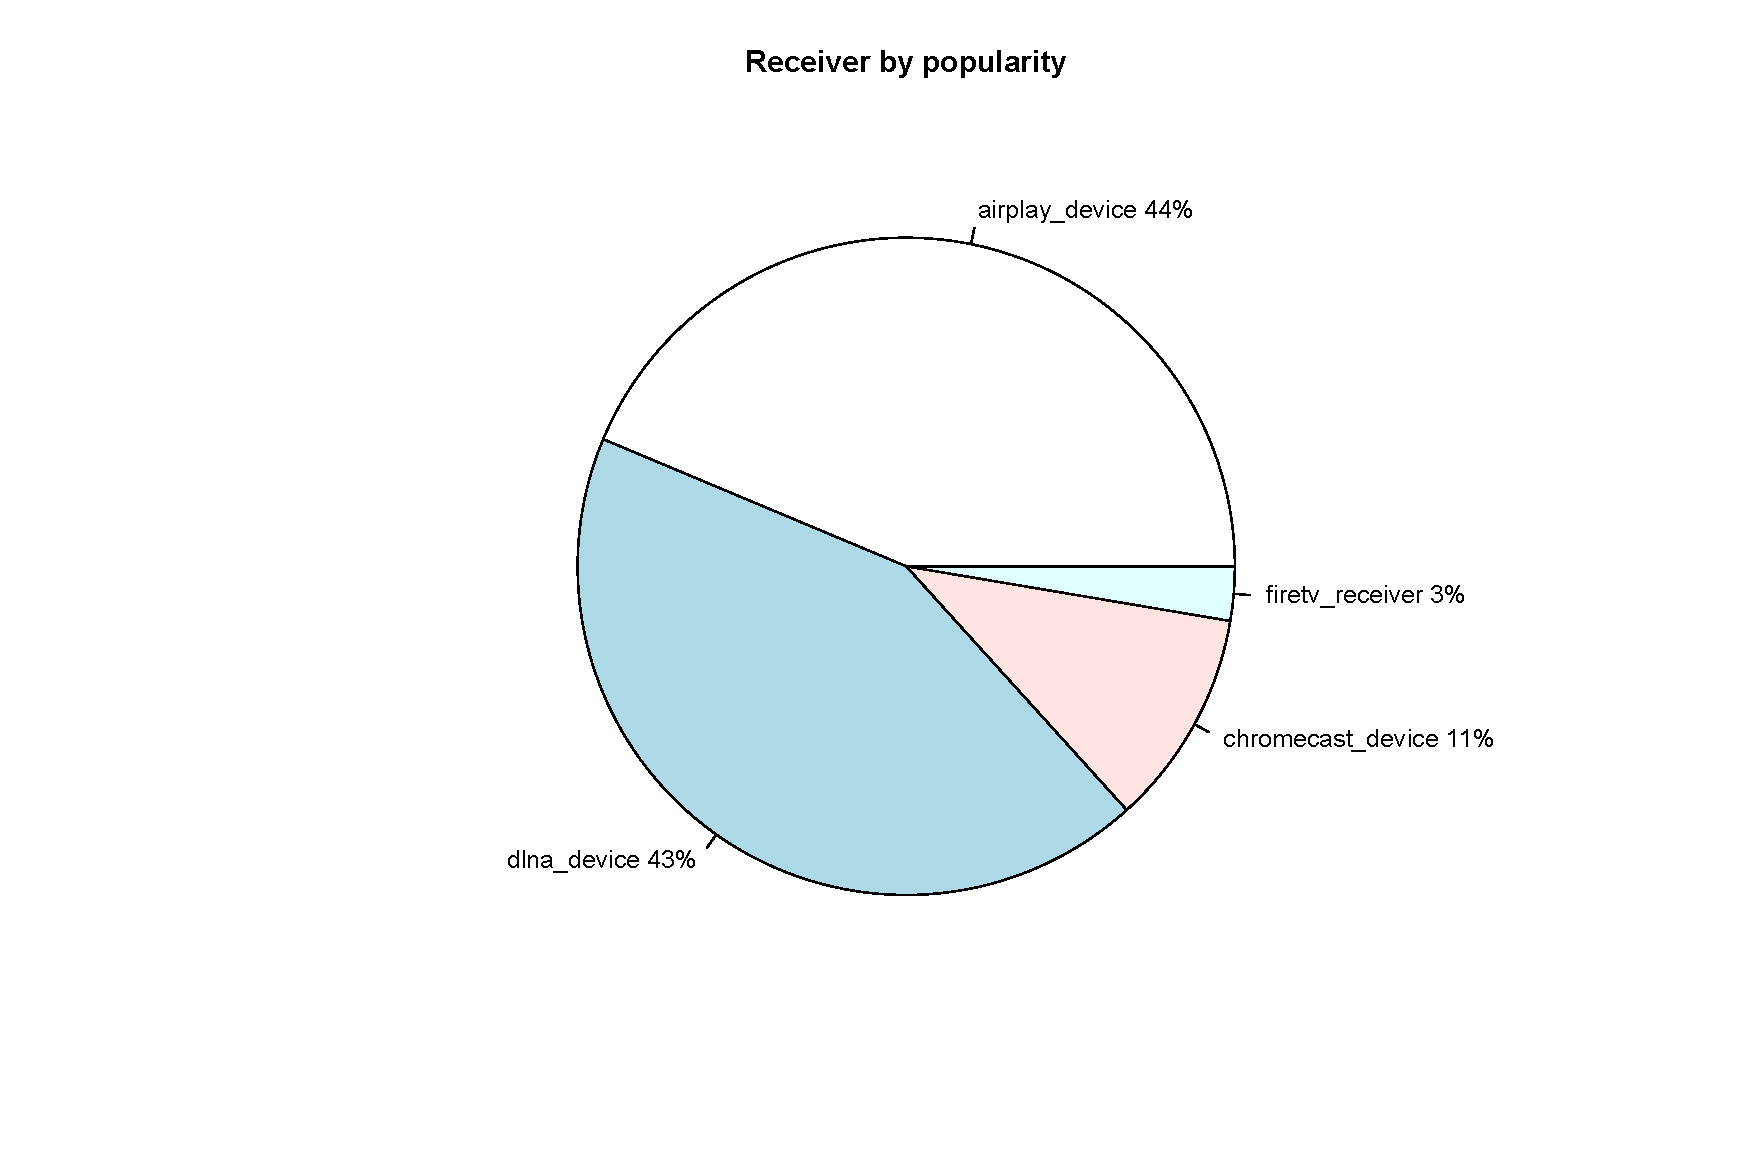
\includegraphics[height=8.5cm]{charts/receiver_popularity}
\caption{Popularity of receiver types \label{receiver_types}}
\end{figure}
\begin{figure}[hb]
\centering 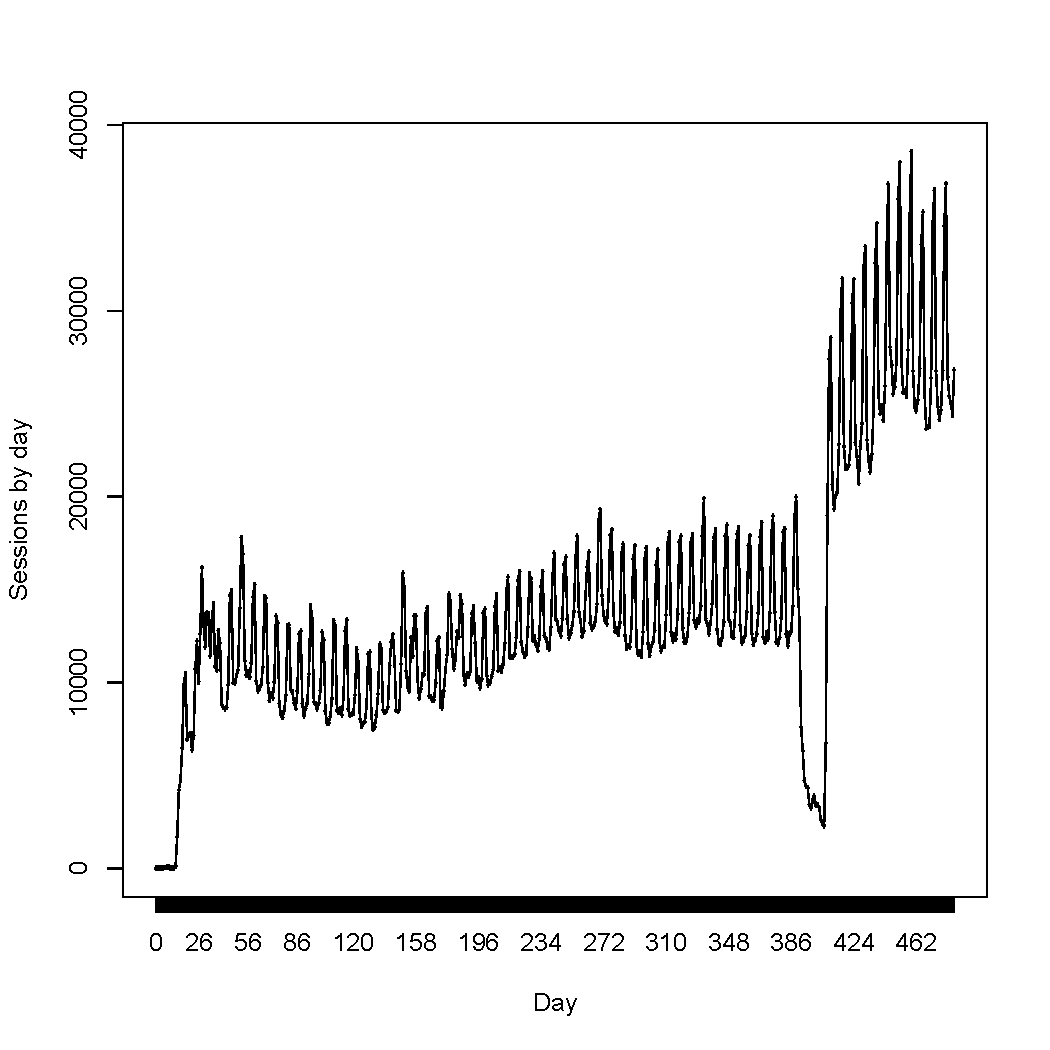
\includegraphics[height=8.5cm]{charts/sessions_per_day}
\caption{Sessions per day \label{sessions_perday}}
\end{figure}
Our application has gone public for 16 months and it has seen a series of small updates and one major update on last Christmas. The number of daily visits is shown in Figure \ref{sessions_perday}. As shown in the figure, after the release, the number of users has seen a great increase in the first two months. After that, the number of active users has remained steady over the following six months, until we launched a major release after around a year. The new release included an updated UI and a better written streaming component. This release has brought a significant growth in users. Currently our application is hitting 15000 visits per day,  proving that our solution has been successful.


\subsection{User study}
It is essential to listen to feedback from users and our application users can send their feedback to us in many ways, such as commenting on the Google Play Store or sending E-mail directly to us.\\
\\
Having been collecting user feedbacks for over 16 months, we have made several improvements accordingly. Most of the feedbacks are about trouble shooting. For example, device discovery problem has been the most common issue for most complaining users. The reason could be that phones and other receivers are not connected to the same Wi-Fi network, or the receivers are not turned on. With more and more user feedback collected, we felt obliged to set up a website for trouble shooting. After the setup of the feedback website we kept updating and improving the trouble shooting pages. Now most complaining users could find their answer in this trouble shooting pages.
